% !TeX program = pdflatex
\documentclass[tikz,border=8pt]{standalone}
\usepackage{tikz}\usetikzlibrary{angles,quotes,calc}
\definecolor{FigureBlue}{HTML}{2563EB}\definecolor{FigureOrange}{HTML}{EA580C}
\begin{document}
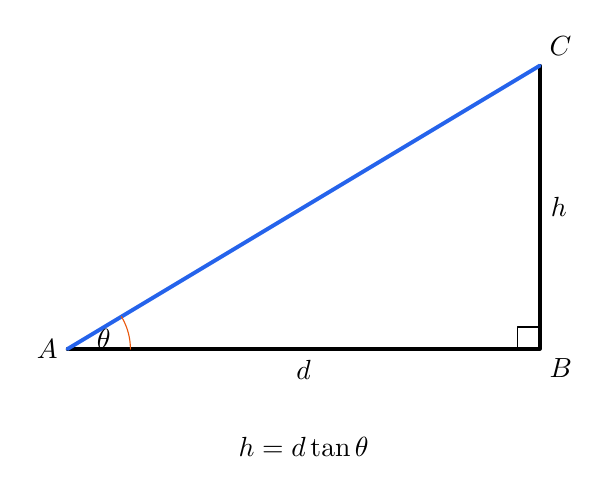
\begin{tikzpicture}[line cap=round,line join=round]
  \coordinate (A) at (0,0); \coordinate (B) at (6,0); \coordinate (C) at (6,3.6);
  \draw[line width=1.2pt] (A)--node[below] {$d$}(B)--node[right] {$h$}(C);
  \draw[FigureBlue,line width=1.4pt] (A)--(C); \draw (B) rectangle ++(-.28,.28);
  \pic[draw=FigureOrange,angle radius=8mm,"$\theta$"] {angle=B--A--C};
  \node[left] at (A) {$A$}; \node[below right] at (B) {$B$}; \node[above right] at (C) {$C$};
  \node[below=10mm] at ($(A)!.5!(B)$) {$h=d\tan\theta$};
\end{tikzpicture}
\end{document}
